%\documentclass[11pt,epsf]{article}
\documentclass[oneside, a4paper, onecolumn, 11pt]{article}

\usepackage{graphicx, amssymb, multicol, amsmath}
\usepackage{fancyhdr, hyperref, sidecap}
\usepackage[left=2.05cm,top=2.05cm,bottom=1.55cm,right=2.05cm]{geometry}
\usepackage[utf8]{inputenc}
\usepackage{natbib}	        %%  bibliography style
\setlength{\bibsep}{0.0pt}
\usepackage{eurosym}
\usepackage{enumitem}
\usepackage{nopageno}
\usepackage{fancyhdr}
\usepackage[usenames,dvipsnames,svgnames,table]{xcolor}


\usepackage{amsmath, amssymb}
\usepackage{booktabs, bm}           %%  bold math
\usepackage{cancel}
\usepackage{dcolumn}  %%  Align table columns on decimal point
\usepackage{epsfig, epsf, eurosym, enumitem}
\usepackage{fancyhdr}
\usepackage[T1]{fontenc}
\usepackage[para]{footmisc}
\usepackage{graphicx }
%\usepackage{lscape}
\usepackage{hyperref,ifthen}
\usepackage{mathptmx, multicol}
\usepackage[authoryear, round]{natbib}
\usepackage{nopageno}
\usepackage{subfigure}
\usepackage{verbatim}
\usepackage{threeparttable}
\usepackage[usenames,dvipsnames]{xcolor}
\usepackage{tcolorbox}
\usepackage{tabularx}
\usepackage{array}
\usepackage{colortbl}
\usepackage{framed}
\usepackage{todonotes}



%%%%%%%%%%%%%%%%%%%%%%%%%%%%%%%%%%%%%%%%%%%
%       define Journal abbreviations      %
%%%%%%%%%%%%%%%%%%%%%%%%%%%%%%%%%%%%%%%%%%%
\def\nat{Nat} \def\apjl{ApJ~Lett.} \def\apj{ApJ}
\def\apjs{ApJS} \def\aj{AJ} \def\mnras{MNRAS}
\def\prd{Phys.~Rev.~D} \def\prl{Phys.~Rev.~Lett.}
\def\plb{Phys.~Lett.~B} \def\jhep{JHEP}
\def\npbps{NUC.~Phys.~B~Proc.~Suppl.} \def\prep{Phys.~Rep.}
\def\pasp{PASP} \def\aap{Astron.~\&~Astrophys.} \def\araa{ARA\&A}
\def\jcap{\ref@jnl{J. Cosmology Astropart. Phys.}} 
\def\nar{New~A.R.} \def\aapr{A\&ARv}

\newcommand{\preep}[1]{{\tt #1} }

%%%%%%%%%%%%%%%%%%%%%%%%%%%%%%%%%%%%%%%%%%%%%%%%%%%%%
%              define symbols                       %
%%%%%%%%%%%%%%%%%%%%%%%%%%%%%%%%%%%%%%%%%%%%%%%%%%%%%
\def \Mpc {~{\rm Mpc} }
\def \Om {\Omega_0}
\def \Omb {\Omega_{\rm b}}
\def \Omcdm {\Omega_{\rm CDM}}
\def \Omlam {\Omega_{\Lambda}}
\def \Omm {\Omega_{\rm m}}
\def \ho {H_0}
\def \qo {q_0}
\def \lo {\lambda_0}
\def \kms {{\rm ~km~s}^{-1}}
\def \kmsmpc {{\rm ~km~s}^{-1}~{\rm Mpc}^{-1}}
\def \hmpc{~\;h^{-1}~{\rm Mpc}} 
\def \hkpc{\;h^{-1}{\rm kpc}} 
\def \hmpcb{h^{-1}{\rm Mpc}}
\def \dif {{\rm d}}
\def \mlim {m_{\rm l}}
\def \bj {b_{\rm J}}
\def \mb {M_{\rm b_{\rm J}}}
\def \mg {M_{\rm g}}
\def \mi {M_{\rm i}}
\def \qso {_{\rm QSO}}
\def \lrg {_{\rm LRG}}
\def \gal {_{\rm gal}}
\def \xibar {\bar{\xi}}
\def \xis{\xi(s)}
\def \xisp{\xi(\sigma, \pi)}
\def \Xisig{\Xi(\sigma)}
\def \xir{\xi(r)}
\def \max {_{\rm max}}
\def \gsim { \lower .75ex \hbox{$\sim$} \llap{\raise .27ex \hbox{$>$}} }
\def \lsim { \lower .75ex \hbox{$\sim$} \llap{\raise .27ex \hbox{$<$}} }
\def \deg {^{\circ}}
%\def \sqdeg {\rm deg^{-2}}
\def \deltac {\delta_{\rm c}}
\def \mmin {M_{\rm min}}
\def \mbh  {M_{\rm BH}}
\def \mdh  {M_{\rm DH}}
\def \msun {M_{\odot}}
\def \z {_{\rm z}}
\def \edd {_{\rm Edd}}
\def \lin {_{\rm lin}}
\def \nonlin {_{\rm non-lin}}
\def \wrms {\langle w_{\rm z}^2\rangle^{1/2}}
\def \dc {\delta_{\rm c}}
\def \wp {w_{p}(\sigma)}
\def \PwrSp {\mathcal{P}(k)}
\def \DelSq {$\Delta^{2}(k)$}
\def \WMAP {{\it WMAP \,}}
\def \cobe {{\it COBE }}
\def \COBE {{\it COBE \;}}
\def \HST  {{\it HST \,\,}}
\def \Spitzer  {{\it Spitzer \,}}
\def \ATLAS {VST-AA$\Omega$ {\it ATLAS} }
\def \BEST   {{\tt best} }
\def \TARGET {{\tt target} }
\def \TQSO   {{\tt TARGET\_QSO}}
\def \HIZ    {{\tt TARGET\_HIZ}}
\def \FIRST  {{\tt TARGET\_FIRST}}
\def \zc {z_{\rm c}}
\def \zcz {z_{\rm c,0}}


\newcommand{\sqdeg}{deg$^{-2}$}
\newcommand{\lya}{Ly$\alpha$\ }
%\newcommand{\lya}{Ly\,$\alpha$\ }
\newcommand{\lyaf}{Ly\,$\alpha$\ forest}
%\newcommand{\eg}{e.g.~}
%\newcommand{\etal}{et~al.~}
\newcommand{\cii}{C\,{\sc ii}\ }
\newcommand{\ciii}{C\,{\sc iii}]\ }
\newcommand{\civ}{C\,{\sc iv}\ }
\newcommand{\SiIV}{Si\,{\sc iv}\ }
\newcommand{\mgii}{Mg\,{\sc ii}\ }
\newcommand{\feii}{Fe\,{\sc ii}\ }
\newcommand{\feiii}{Fe\,{\sc iii}\ }
\newcommand{\caii}{Ca\,{\sc ii}\ }
\newcommand{\halpha}{H\,$\alpha$\ }
\newcommand{\hbeta}{H\,$\beta$\ }
\newcommand{\oi}{[O\,{\sc i}]\ }
\newcommand{\oii}{[O\,{\sc ii}]\ }
\newcommand{\oiii}{[O\,{\sc iii}]\ }
\newcommand{\heii}{[He\,{\sc ii}]\ }
\newcommand{\nii}{N\,{\sc ii}\ }
\newcommand{\nv}{N\,{\sc v}\ }

%% From:: /cos_pc19a_npr/LaTeX/proposals/JWST/JWST_ERS/Proposal/lines.tex
%%  
\newcommand{\imw}{$i$--$W3$}
\newcommand{\imwf}{$i$--$W4$}
\newcommand{\rmwf}{$r$--$W4$}
\newcommand{\imwt}{$i$--$W2$}
\newcommand{\wtmwf}{$W3$--$W4$}
%\newcommand{\kms}{km s$^{-1}$}
\newcommand{\cmN}{cm$^{-2}$}
\newcommand{\cmn}{cm$^{-3}$}
%\newcommand{\msun}{M$_{\odot}$}
\newcommand{\lsun}{L$_{\odot}$}
\newcommand{\lam}{$\lambda$}
\newcommand{\mum}{$\mu$m}
\newcommand{\ebv}{$E(B$$-$$V)$}
%\newcommand{\heii}{\mbox{He\,{\sc ii}}}
\newcommand{\cv}{\mbox{C\,{\sc v}}}
%\newcommand{\civ}{\mbox{C\,{\sc iv}}}
%\newcommand{\ciii}{\mbox{C\,{\sc iii}}}
%\newcommand{\cii}{\mbox{C\,{\sc ii}}}
%\newcommand{\nv}{\mbox{N\,{\sc v}}}
\newcommand{\niv}{\mbox{N\,{\sc iv}}}
\newcommand{\niii}{\mbox{N\,{\sc iii}}}
%\newcommand{\oi}{\mbox{O\,{\sc i}}}
%\newcommand{\oii}{\mbox{O\,{\sc ii}}}
%\newcommand{\oiii}{\mbox{[O\,{\sc iii}]}}
\newcommand{\oiv}{\mbox{O\,{\sc iv}}}
\newcommand{\ov}{\mbox{O\,{\sc v}}}
\newcommand{\ovi}{\mbox{O\,{\sc vi}}}
\newcommand{\ovii}{\mbox{O\,{\sc vii}}}

%\newcommand{\feii}{\mbox{Fe\,{\sc ii}}}
%\newcommand{\feiii}{\mbox{Fe\,{\sc iii}}}
%\newcommand{\mgii}{\mbox{Mg\,{\sc ii}}}
\newcommand{\neii}{[Ne\,{\sc ii}]\ }
\newcommand{\neiii}{[Ne\,{\sc ii}]\ }
\newcommand{\nev}{Ne\,{\sc v}\ }
\newcommand{\nevi}{[Ne\,{\sc vi}]\ }
\newcommand{\neviii}{\mbox{Ne\,{\sc viii}}}
\newcommand{\aliii}{\mbox{Al\,{\sc iii}}}
\newcommand{\siii}{\mbox{Si\,{\sc ii}}}
\newcommand{\siiii}{\mbox{Si\,{\sc iii}}}
\newcommand{\siiv}{\mbox{Si\,{\sc iv}}}
%\newcommand{\lya}{\mbox{Ly$\alpha$}}
%\newcommand{\lyb}{\mbox{Ly$\beta$}}
\newcommand{\hi}{\mbox{H\,{\sc i}}}
\newcommand{\snine}{\mbox{[S\,{\sc ix}]}}
\newcommand{\sivi}{\mbox{[Si\,{\sc vi}]}}
\newcommand{\sivii}{\mbox[{Si\,{\sc vii}]}}
\newcommand{\siix}{\mbox{[Si\,{\sc ix}]}}
\newcommand{\six}{\mbox{[Si\,{\sc x}]}}
\newcommand{\sixi}{\mbox{[Si\,{\sc xi}]}}
\newcommand{\caviii}{\mbox{[Ca\,{\sc viii}]}}
\newcommand{\arii}{\mbox{[Ar\,{\sc ii}]}}

%%[Ar II] 6.97
%% [S IX] 1.252 μm 328 
% [Si X] 1.430 μm 351 
% [Si XI] 1.932 μm 401 
% [Si VI] 1.962 μm 167 
% [Ca VIII] 2.321 μm 128 
% [Si VII] 2.483 μm 205 
% [Si IX] 3.935 μm 303
% [Ar II] 6.97


%\snine\ at 1.252$\mu$m, \six\ at 1.430$\mu$m, \sixi\ at 1.932$\mu$m, \sivi\ at
%1.962$\mu$m, \caviii\ at 2.321$\mu$m, \sivi\ at 2.483$\mu$m \siix\ at
%3.935$\mu$m and \arii\ at 6.97$\mu$m. 
%%
%% such as [Ne ii]12.8 μm, [Ne v]14.3 μm, [Ne iii]15.5 μm, [S iii]18.7 μm and 33.48 μm, [O iv]25.89 μm and [Si ii]34.8 μm (e.g
%%
%% MIR emission lines like [NeII] and [NeV] are ..
%%
%% Also,  arXiv:astro-ph/0003457v1 
%% [NeV] 14.32um & 24.32um and [NeVI] 7.65um imply an A(V)>160 towards the NLR...
%% [NeIII]15.56um/[NeII]12.81um
%%
%% [Ne V] 14.3, 24.2 μm 97.
%% [Ne II] 12.8 μm
%% [OIV] 26μm
%%


%% To fix list things: 
\setitemize{noitemsep,topsep=0pt,parsep=0pt,partopsep=0pt,leftmargin=*}
\renewcommand{\labelitemi}{\tiny$\blacksquare$}

\pagestyle{fancy}
\renewcommand{\headrulewidth}{0pt}  %% Remove line at top

%\pagestyle{empty}
\fancyhf{}
%\lhead{{\it ERC-2015-StG}}
%\lhead{{\it DEQUASARS: Part B1 }}
\lhead{{\it Ross}}
\chead{{\it MIQSOs}}
\rhead{Part B1.a}
\setcounter{page}{1}
\lfoot{{\it ERC-2015-StG}}
\rfoot{{\it Extended Synopsis}}
\cfoot{{\it Page \thepage\ of 5}}
%\rfoot{{\it FP7-PEOPLE-2013-IIF}}

\newenvironment{itemize*}%
  {\begin{itemize}%
    \setlength{\itemsep}{0pt}%
    \setlength{\parskip}{0pt}}%
  {\end{itemize}}


\begin{document}

\begin{center}
 {\Large \bf \textcolor{Cerulean}{Using Quasars to establish and kickstart \\}}
\vspace{4pt} 
  {\Large \bf \textcolor{Cerulean}{the new field of Extragalactic Variable Astrophysics} }
\end{center}

\begin{quotation}
\noindent
{\it 
Our ERC Consolidator grant proposal will radically improve our understanding of 
one of the two fundamental energy sources available to galaxies; that of accretion 
onto the compact object in the central engine. We will achieve this by leveraging 
several of the new, large-scale surveys that are coming online in the next few years. 
The scope and remit of an ERC Consolidator grant will allow us to combine these 
data products in a manner that will 
% This programme will 
not only establish the new state-of-the-art in extragalactic variable science, 
{\rm it will establish and kickstart the new field of extragalactic variable science itself}. 
%%
The P.I. is a world-leader in observational quasar astrophysics, both in terms of 
survey work and individual object study. 
%%
Our proposal takes astrophysics into the 2020s, going from single objects samples, 
to surveys and samples of millions of objects leveraging these multi-billion Euro/dollar/pound  
next generation missions, telescopes and their subsequent datasets. 
%%

\noindent
Quasars are ideal laboratories and tools for
three main lines of investigation: {\rm (i)} to learn about the
physical processes in accretion disks observed on $\lesssim$year
timescales; {\rm (ii)} connecting accreting active galactic nuclei
(AGN) with galaxy evolution and {\rm (iii)} to use quasars as
cosmological probes. 
%%
The goal is to connect the physics invoked here
from sub-parsec to cosmological scales, and to investigate the
physical processes that link luminous AGN activity and the formation
and evolution of massive galaxies. These critical observations are
made by exploiting the large imaging and spectroscopic datasets that
we will have available from the 
SDSS-V, DESI,  4MOST, LSST and ESA Euclid. 
%% 
Here we ask for 3 postdocs, and `buy-in' to two of the surveys. 
}
\noindent
\end{quotation}

%You need to answer 5 key questions: Why bother? , Is this a European priority? , is the solution already available? Why now-what would happen if you did not do this now?, Why you?. You should aim to have these addressed in the first paragraph of your proposal! The “WHY NOW” is one of the most important ones for ERC.

If we are to understand galaxy formation and evolution, we have to understand the two major power sources available to a galaxy; nuclear fusion in stars and accretion onto compact objects. Our proposal directly addresses the latter process. This is 
a worldwide research priority, but is also a European priority, due to the investment in the ESA {\it Euclid} and {\it Gaia} missions, and the developements of new ESO telescopes (ELT) and instrumentation (4MOST). 
(e.g. 
{\bf Also connection to gravitational waves!!!} 

\noindent
{\bf \underline {Background:}}
%{\bfseries \large \textcolor{Cerulean}{Background:}}
%{\bfseries \underline{\textcolor{Cerulean}{Background:}}}
Where do galaxies come from? How do black holes form and grow? And
what is the history, and fate, of the Universe?  These are the
deepest, most fundamental questions in astrophysics and cosmology, and
sets the scene for my research.

\smallskip 
\smallskip
\noindent
We now know that in the local Universe, there is a link between the
key properties of massive galaxies, such as bulge mass, and their
central supermassive black holes (SMBHs; e.g., [1], [2]). This has led
to the proposal that the supermassive black hole, when accreting, has
an influence on its host galaxy by the means of some regulatory
``feedback'' mechanism(s) (e.g., [3], [4]). However, the details of
the physical processes involved in AGN feedback are still disputed
and, moreover, direct observational evidence for AGN feedback in the
early universe is conspicuous by its absence (e.g., [5], [6]). Hence,
a major source of uncertainty in our current understanding of galaxy
evolution is how supermassive black holes influence, and potentially
regulate, their host galaxies.
%%
What is the main AGN triggering mechanism at the height of quasar
activity? What direct observational evidence in individual objects
links AGN activity to star formation?  Can we observe ``AGN feedback''
in action, in situ, for the most luminous sources?  Such unknowns
about the co-evolution of black holes and their host galaxies remain
among the most fundamental unanswered questions in extragalactic
astronomy.


\smallskip 
\smallskip
\noindent
Furthermore, the details of the physical processes involved in the AGN
activity including how the SMBH directly couples and affects its most
local environment, i.e., the accretion disk, broad line region and
dusty torus, are still unknown at this point (e.g., [7], [8]). Noting
- and for the most part, currently ignoring this issue - quasars have
become key cosmological probes; by being high-$z$ tracers of the
underlying matter distribution ([9]) and as ``backlights'' to observe
the IGM (e.g., [10-15]).



%\smallskip \smallskip
\medskip 
\medskip
\noindent
{\bfseries \large \textsc{\textcolor{Cerulean}{Current Research Highlights}}}

\smallskip
\smallskip
\noindent
My current research has involved discovering new types of quasars,
which are proving to be the key laboratories in (a) understanding the
physical processes linking accretion disk physics to the host galaxy
and (b) understanding the physical processes linking quasar activity
to the host galaxy and wider galactic environment.


\smallskip \smallskip
\smallskip
\smallskip
\noindent
%\textbf{\textsc{Extremely Red Quasars: Feedback in action at high-$z$:}}
\textbf{\textsc{Extremely Red Quasars:}}
In [16] I discovered a new class of object, the ``extremely red
quasars'', that have optical spectroscopy from SDSS/BOSS, and
$r-[22\mu{\rm m}]>14$ colors (i.e., $F_{\nu,\, {\rm MIR}} / F_{\nu,\,
{\rm opt}} \gtrsim 1000$) from the Wide-field Infrared Survey Explorer
(WISE; [17]) satellite, see Figure~\ref{fig:ERQ}.  The ERQs are a
unique obscured quasar population with extreme physical conditions
related to powerful outflows across the line-forming regions. These
sources are the signposts of the most dramatic form of quasar feedback
at the peak epoch of galaxy formation, and may represent an active
``blow-out'' phase of quasar evolution ([18], [19]).  However, due to
the current lack of access to mid-infrared spectroscopy, it is still
unknown whether the large IR luminosities observed in these quasars is
from star formation, which would produce strong polycyclic aromatic
hydrocarbon (PAH) spectral features, or, if it is from the hot dust
near the central quasar, which should produce much weaker/no PAH
emission.


\begin{figure}[h]
  \begin{center}
   \hspace{-0.5cm}
%   trim=l b r t
    \includegraphics[height=5.5cm,width=18.0cm] %, trim={0.05cm 0 0.05cm 0},clip]
   {figures/WISE_SDSSzoomHSC_ERQ-image_v3.pdf}
    \vspace{-10pt}
   \caption{%\small   
\footnotesize 
%     \scriptsize
 %    \tiny
The IR and optical imaging of J2323-0100, an archetype of the
``Extremely Red Quasars'' (ERQs) at $z\approx2.5$ and a {\it JWST}
target. Shown are WISE {\it (left)}, where the quasar booms out as
indicated by the arrow; the SDSS image {\it (middle left)} with
zoom-in {\it (middle right)} on the optically faint source, and new
HSC imaging {\it (right)}, which shows tantalizing evidence for a
faint companion galaxy. Optical rest-frame spectra of J2323-0100,
revealed very broad (FWHM = 2500-5000 km s$^{-1}$), strongly
blue-shifted (by up to 1500 km s$^{-1}$) \oiii\ $\lambda$5007\AA\
emission lines in the ERQs. This is suggestive of active outflows and
potentially evidence for AGN feedback in action at the height of SMBH
activity.
}
  \vspace{-12pt}
 \label{fig:ERQ}
\end{center}
\end{figure}


\smallskip \smallskip
\smallskip
\smallskip
\noindent
\textbf{\textsc{SpIES, Telling us about AGN Feedback:}}
My finishing graduate student, John Timlin, is leading the analysis of the {\it
Spitzer}-IRAC Equatorial Survey (SpIES; [20]), which is a new deep
3.6$\mu$m and 4.5$\mu$m imaging survey designed to discover obscured
and faint unobscured quasars in the SDSS Stripe 82 field. The
scientific goals of SpIES are to measure the quasar luminosity
function and clustering to $z\sim4$, and potentially discover a suite
of very high redshift quasars, meanwhile constraining AGN ``feedback''
models.  In [21] we made the first measurements of clustering of
IR-selected $z > 3$ AGNs.  Connecting to current lower-$z$
measurements, we find an ``inefficient feedback'' model is favored,
where all $z>2$ BHs grow to their peak luminosity at $z\sim2$ and then
fully ``shut down'' ($\dot{m}_{\rm accr} \leq 10^{-5}~M_{\odot}$~yr$^{-1}$).


\smallskip \smallskip
\smallskip
\smallskip
\noindent
%\textbf{\textsc{Changing-Look Quasars:}}
\textbf{\textsc{A microscope for rapid Central Engines:}}
Recently ``Changing-look'' quasars (CLQs; [22-25]) have been
identified, and are defined to be luminous AGN which have a dramatic
appearance, or disappearance, of their broad emission-line component
on observed-frame month-to-year timescales.  CLQs are important since
they offer a direct observational probe into the physical processes
dictating the structure of the broad-line region (BLR). These
timescales can potentially be associated with the viscous timescale
(the drift time through the accretion disk), the light crossing
timescale (critical for reverberation mapping and disk reprocessing)
and the dynamical timescale of the BLR.  CLQs are thus an ideal
laboratory for studying accretion physics, as the entire system
responds to a large change in ionizing flux on a human timescale.

\smallskip \smallskip
\noindent 
In [25] I co-led the first systematic search for CLQs based on
photometry from SDSS and Pan-STARRS1, along with repeat spectra from
the SDSS/BOSS, and reported the discovery of 10 CLQs. This is a
startling result since we now estimate $\approx$10-15\% of bona fide
quasars may exhibit `changing look' behaviour on $\sim$10 year 
(rest-frame) timescales. However, plausible time-scales for variable
dust extinction are factors of $2-10$ too long to explain the dimming
and brightening in these sources.  Changes in accretion rate are the
currently favored explanation for CLQs, but then the question of how
the inner accretion disk couples to the BLR immediately
arises. Further investigation is thus warranted.



%\smallskip \smallskip
\medskip\medskip
\noindent
%{\bf \large \underline{Future Research}}
{\bfseries \large \textsc{\textcolor{Cerulean}{Future Research}}}

\smallskip
\smallskip
\noindent
My future research builds on, and expands my current research program;
I have a bold research vision that is designed to be addressed by a
research group, and the environment, current research areas and
telescope access in the Department of Physics and Astronomy at Dartmouth College
are ideal to
carry out these investigations.
%%
The science questions we seek to address are well-posed, yet strike at
the heart of major and still open extragalactic astrophysical
questions: Do we have a full accounting for the accretion history in
the Universe?  How does the energy `escape' from the central engine to
the host galaxy?  Are the modes of AGN ``feedback'' that regulate a
galaxy the same that regulate the AGN itself?  What are the
star-formation properties of mid-infrared luminous quasars at the peak
of quasar activity?  What are the evolutionary properties, if any, of
dark energy?


\smallskip \smallskip
\smallskip
\smallskip
\noindent
\textbf{\textsc{New IR investigations into the CLQ Population:}}
Taking advantage of new optical imaging data from the Dark Energy
Camera Legacy Survey \href{http://legacysurvey.org/decamls/}{(DECaLS)}
and new IR light-curves from NEOWISE ([26, 27]), we have made further
in-roads into understanding the CLQ population. This includes
identifying objects with rapidly changing IR light-curves and also
accretion disk changes, e.g. the $z=0.378$ quasar SDSS
J110057-005304.4, see Figure~\ref{fig:J110057}. From J110057, my new
model ([28]) suggests a dramatic new picture of the physics of the
CLQs governed by processes at the innermost stable circular orbit
(ISCO) and the structure of the innermost disk. {\it We have embarked
on a new observation campaign, gaining optical light-curves (from the
Liverpool Telescope) and spectra (from WHT and Palomar) to test this
startling new hypothesis.}
\begin{figure}[h]
  \begin{center}
    \hspace{-0.5cm}
    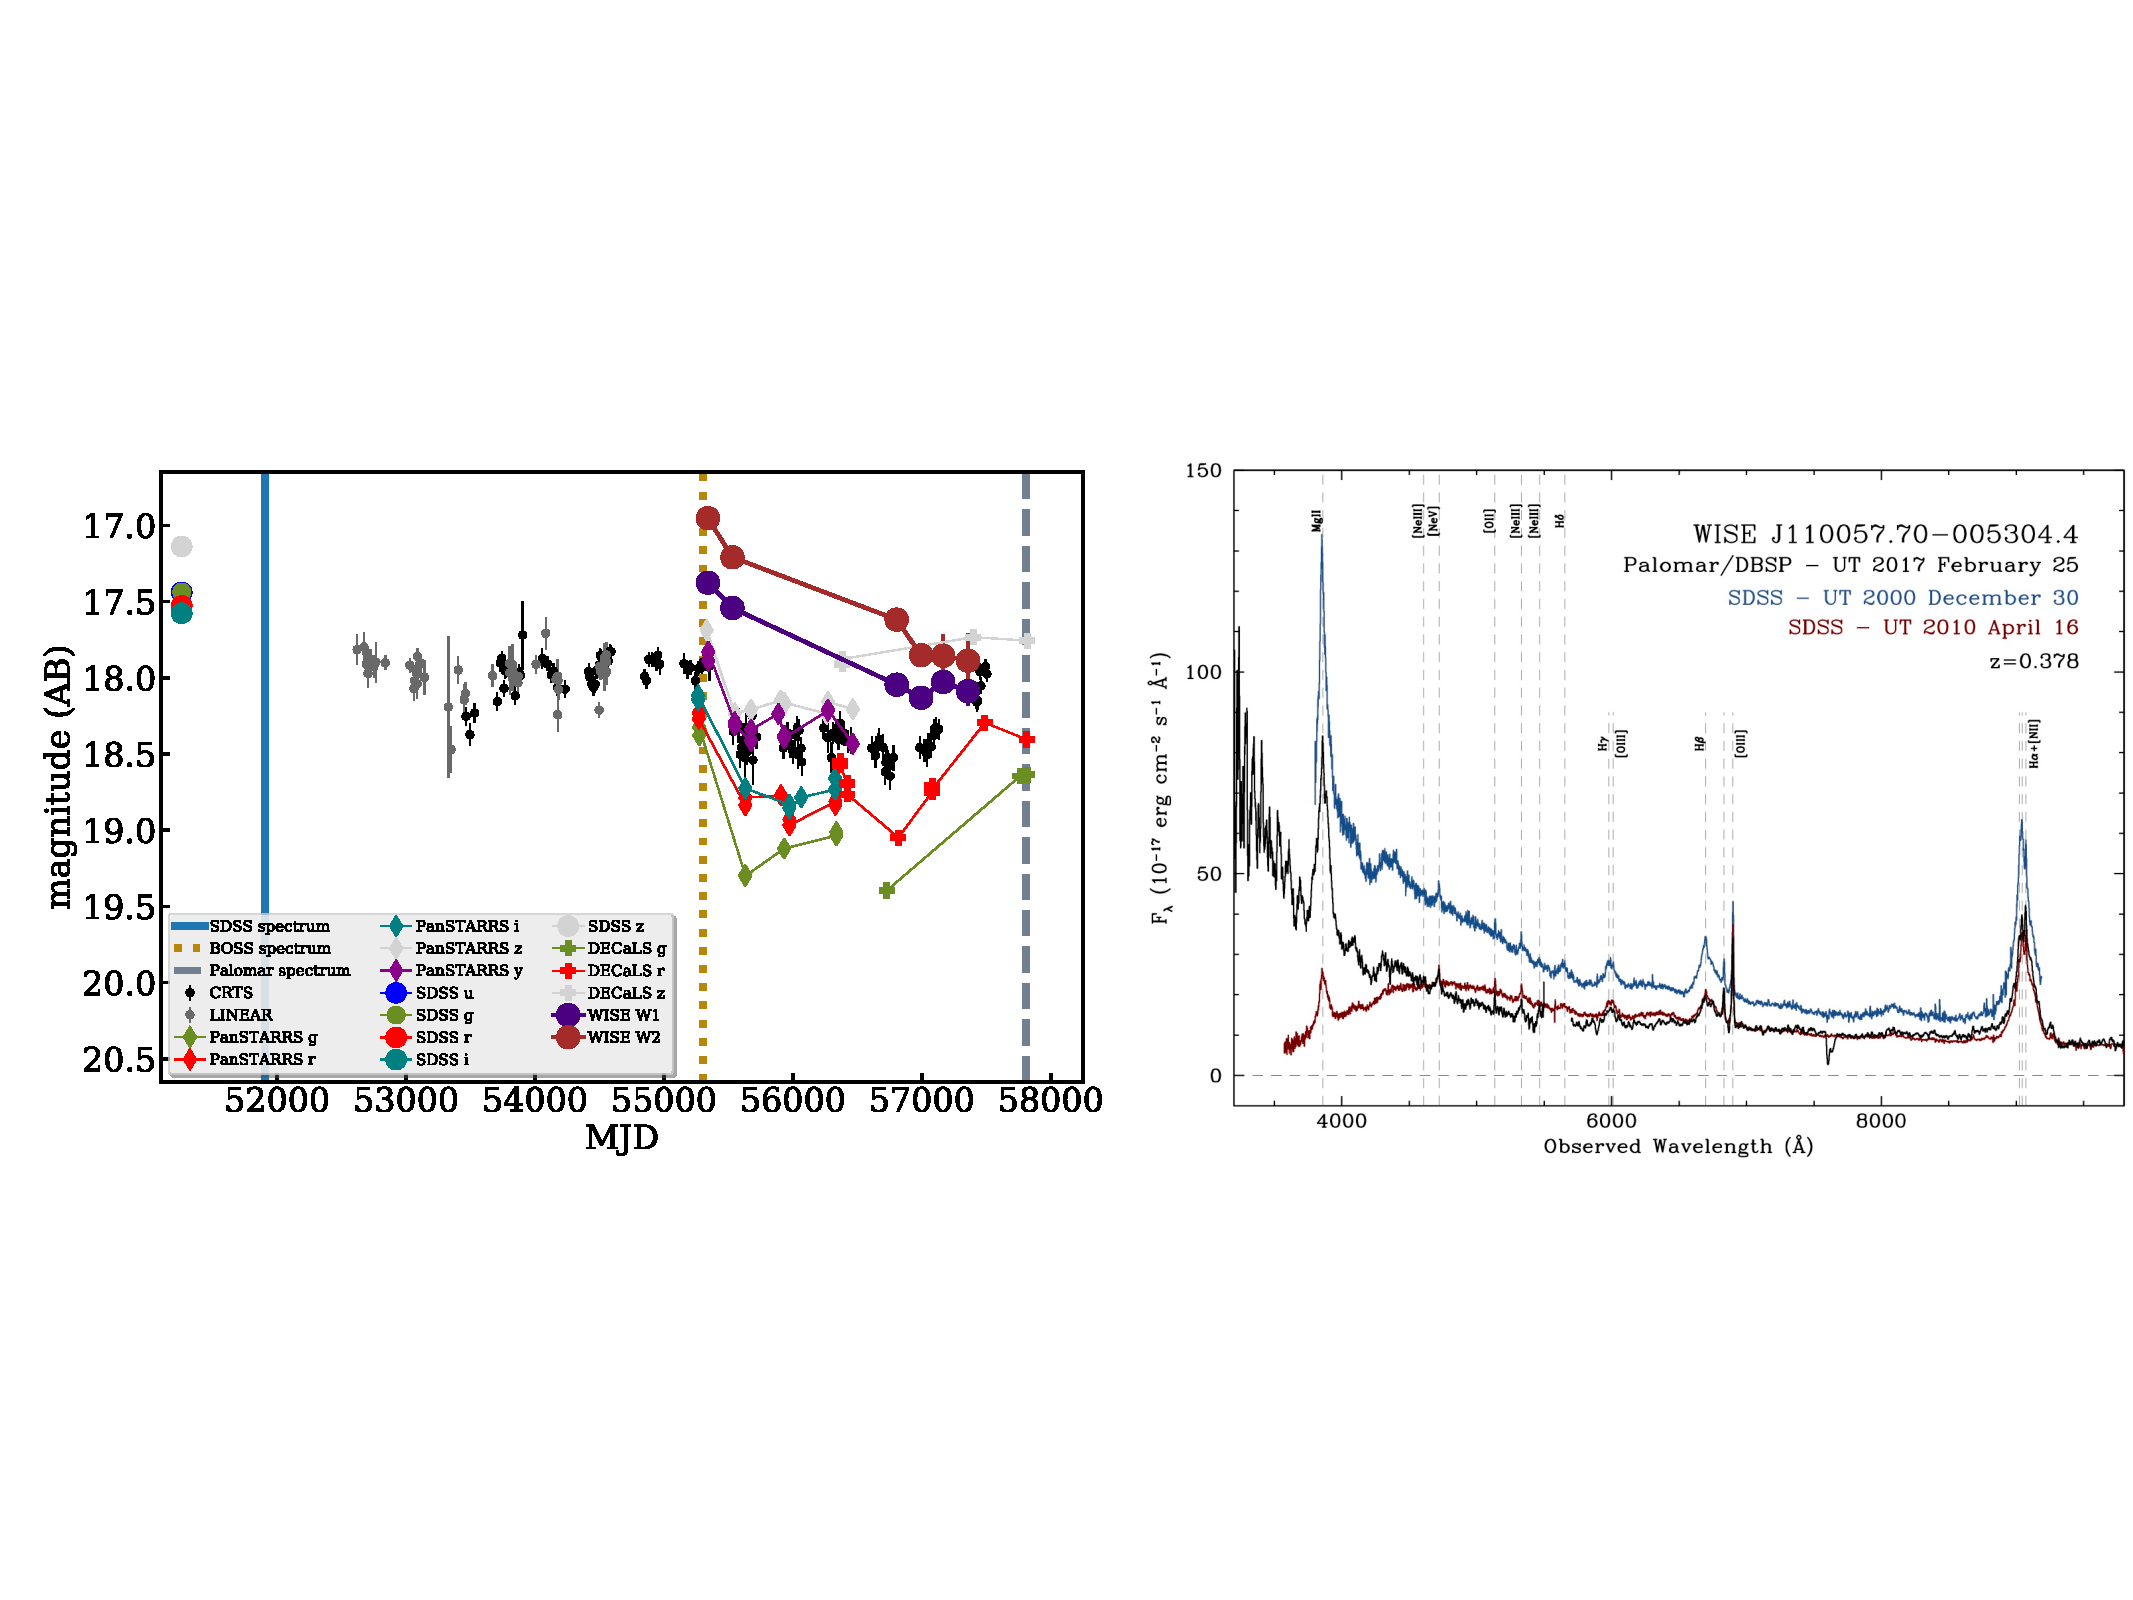
\includegraphics[height=6.25cm,width=17.2cm]
    {figures/J110057_LC_Spectra_20171024.pdf}
    \vspace{-10pt}
    \caption{%\small      
      \footnotesize 
      % \scriptsize
      % \tiny
      {\it (Left:)} The optical and infrared light-curve for J110057; 
      Note the fall in the infrared, whereas there is a decrease, but 
      then recovery in the optical. 
      {\it (Right:)} 
      Three epochs of spectra for J110057. 
      The spectacular downturn in the blue for the 2010 spectrum 
      indicates a dramatic change in the accretion disk.
    }
  \vspace{-16pt}
 \label{fig:J110057}
\end{center}
\end{figure}


\smallskip \smallskip
\smallskip \smallskip
\noindent
\textbf{\textsc{Early Science with the James Webb Space Telescope: }}
The {\it James Webb Space Telescope} ({\it JWST}) is a 6.5-meter
infrared telescope that will initiate and enable transformative
science. My discovery of the extremely red quasars provides a key
observational clue to the ``major merger'' evolutionary theory for
quasar activity ([29]). I am the P.I. of a large, multi-proposal Cycle 1
programme, that will take maximal advantage of {\it JWST's} new and
uniquely powerful capabilities immediately upon commencing science
operations. The natural science case for {\it JWST} is the detailed
investigation of the incredible richness of the near- and mid-IR spectral
features in the ERQs using the NIRSpec and MIRI spectrographs, and by
utilizing my experience with mid-infrared datasets, surveys and object
discovery, I am leading a team of postdocs and graduate students, to
carry out these investigations. {\it The next JWST Call for Proposals
is in December 2017, and my team is ramping up for a full suite of ERQ
related proposals for this truly revolutionary mission}.


\smallskip \smallskip
\smallskip
\smallskip
\noindent
\textbf{\textsc{Quasars, Dark Energy and Very Wide Field Surveys: }}
In the community's future is the prospect of very wide-field
ground-based surveys using both imaging and spectroscopy, in the North
and Southern Hemisphere. Building on {\it (i)} my leadership
experience and heritage from being an integral part of BOSS and {\it
(ii)} my world-leading expertise in quasar target selection,
demographics, and physical properties, I will continue to lead the
scientific development of using quasars as large-scale structure (LSS)
tracers in these new surveys.

\smallskip \smallskip
\noindent 
%{\bf \underline {Outline of Future Research:}}
Prior to SDSS-III BOSS, quasars lagged behind massive galaxies as good
tracers of LSS. However, with the evolution of Baryon Acoustic
Oscillation (BAO) and Redshift-Space Distortion (RSD) studies using
BOSS, and in particular the Lyman-$\alpha$ forest (Ly$\alpha$F),
quasars are now seen as key objects in accessing the high-$z$
Universe. Moreover, in the DESI era, there is huge potential to extend
this reach further, first for BAO/RSD and also as Standard Candles. 


\begin{itemize}
\item{{\bf Quasars as Cosmological Probes {\sc I:} Baryon Acoustic
      Oscillations.} I co-led the first investigation that successfully used
    quasars as point test particles to measure the BAO signature
    [15]. This measurement was a cross-correlation with the Ly$\alpha$F,
    but demonstrated that quasars themselves, despite their lower number
    density can trace LSS sufficiently well for BAO studies. This
    provides access to geometry measurements at $z>1$, further
    constraining the Hubble Parameter at high-$z$ and testing the current
    $\Lambda$CDM model.  {\it DESI will be ``the ultimate quasar survey'',
      with sub-per cent measurements of the distance scale (from BAO alone)
      to redshifts of $z\sim3$ using `tracer' and Ly$\alpha$F quasars.}}
  
\item{{\bf Quasars as Cosmological Probes {\sc II:} RSDs with
      Quasars.}  As I proved with the original SDSS sample ([31]), quasars
    can also be used to measure RSDs.  Measurements of the normalized
    growth rate, $f\sigma_{8}$, from RSD using quasars at $z\sim1.5$ is
    crucial since model predictions diverge at these redshifts for
    $\Lambda$CDM+G.R. compared to $f(R)$ gravity, DGP braneworld, and varying
    Gravitational Constant models ([32, 33]). {\it Even with the local
      GW170817 measurements, a range of gravity theories persist and
      testing General Relativity at cosmological scales remains imperative.}}
  
\item{{\bf Quasars as Cosmological Probes {\sc III:} Reverberation
      Mapping Campaigns.}  Recently, [34-37] demonstrated that by using the
    tight relationship between the luminosity of a quasar and the radius
    of its broad-line region, established via reverberation mapping, one
    is able to determine the luminosity distances to quasars.  This means
    that quasars can now be used as standard, or more accurately,
    ``standardizable'' candles (in a very similar way to Type Ia
    supernovae). {\it Thus with light-curve data from LSST and a baseline
      for repeat spectroscopy from SDSS, DESI is ideally placed to exploit
      this new method, with very different systematics to the BAO, and
      access a redshift regime $z>4$ where even the Ly$\alpha$F will not be
      able to offer cosmology constraints.}}

\end{itemize}


%\input{Why}


\begin{center}
\medskip
 \medskip
 {\large \bf References}
    \vspace{-10pt}
\end{center}
\begin{multicols}{3}[]
\noindent
%\footnotesize
\scriptsize
%\tiny
\lbrack 1\rbrack Kormendy \& Ho, 2013, ARAA, 51, 511\\
\lbrack 2\rbrack Kormendy,  2016, ASSL, 418, 431\\
\lbrack 3\rbrack Alexander et al., 2012, NewAR, 56, 93\\
\lbrack 4\rbrack King \& Pounds, 2015, ARAA, 53, 115 \\
\lbrack 5\rbrack Heckman \& Best, 2014, ARAA, 52, 589\\
\lbrack 6\rbrack Naab \& Ostriker, 2017, ARAA, 55, 59 \\
\lbrack 7\rbrack Netzer, 2015, ARAA, 53,  365\\
\lbrack 8\rbrack Padovani, 2017, A\&ARv, 25, 2\\
%%
\lbrack  9\rbrack Ata et al., 2017, arXiv1705.06373v2\\
\lbrack10\rbrack Solsar et al., 2013, JCAP, 04, 026 \\
\lbrack11\rbrack Busca et al.,  2013, A\&A, 552, 96 \\
\lbrack12\rbrack Delubac et al.,  2015, A\&A, 574, 59 \\
\lbrack13\rbrack Bautista et al., 2017, A\&A, 603, 12 \\
\lbrack14\rbrack du Mas des Bourboux et al., 2017, arXiv1708.02225v3\\
\lbrack15\rbrack Font-Riber et al., 2014, JCAP, 05, 027\\
%%
\lbrack16\rbrack Ross et al. 2015, MNRAS, 453, 3932\\
\lbrack17\rbrack Wright et al., 2010, AJ, 140, 1868\\
\lbrack18\rbrack Zakamska et al., 2016, MNRAS, 459, 3144\\
\lbrack19\rbrack Hamann et al., 2017, MNRAS, 464, 3431\\
%%
\lbrack20\rbrack Timlin, Ross et al., 2016, ApJS, 225, 1\\
\lbrack21\rbrack Timlin, Ross et al., 2017, ApJ, {\it in prep.}\\
%%
\lbrack22\rbrack LaMassa et al., 2015, ApJ, 800, 144\\
\lbrack23\rbrack Runnoe et al., 2016, MNRAS, 455, 1691\\
\lbrack24\rbrack Ruan et al, 2016, ApJ, 826, 188\\
\lbrack25\rbrack MacLeod, Ross et al., 2016, MNRAS, 457, 389\\
%%
\lbrack26\rbrack Meisner et al., 2017, AJ, 153, 38 \\
\lbrack27\rbrack Meisner et al., 2017, AJ, 154, 161 \\
% Meisner  et al., 2017, arXiv1710.02526v1 \\
\lbrack28\rbrack Ross et al., 2017, Nat.As., {\it in prep.} \\
%%
\lbrack29\rbrack Hopkins et al., 2006, ApJS, 163, 1\\
%%
\lbrack30\rbrack Schlegel et al., 2011,  arXiv:1106.1706v2 \\
%
\lbrack31\rbrack Ross et al., 2009, ApJ, 697, 1634 \\
%%
\lbrack32\rbrack Lombriser \& Taylor, 2016, JCAP, 03, 031 \\
\lbrack33\rbrack Baker et al, 2017,  arXiv1710.06394v1 \\
%%
\lbrack34\rbrack Watson et al.,  2011, ApJ, 740, L49\\
\lbrack35\rbrack King et al., 2014, MNRAS, 441, 3454\\
\lbrack36\rbrack King et al., 2015, MNRAS, 453, 1701\\
\lbrack37\rbrack Shen et al., 2015, ApJS, 216, 4\\
%\lbrack37\rbrack The Pierre Auger Collaboration, 2017, Science, 357, 6357 \\
\lbrack38\rbrack Hviding et al.,  2017, arXiv1711.01269v1 



\end{multicols}



\end{document}
